% 
% Annual Cognitive Science Conference
% Sample LaTeX Paper -- Proceedings Format
% 

% Original : Ashwin Ram (ashwin@cc.gatech.edu)       04/01/1994
% Modified : Johanna Moore (jmoore@cs.pitt.edu)      03/17/1995
% Modified : David Noelle (noelle@ucsd.edu)          03/15/1996
% Modified : Pat Langley (langley@cs.stanford.edu)   01/26/1997
% Latex2e corrections by Ramin Charles Nakisa        01/28/1997 
% Modified : Tina Eliassi-Rad (eliassi@cs.wisc.edu)  01/31/1998
% Modified : Trisha Yannuzzi (trisha@ircs.upenn.edu) 12/28/1999 (in process)
% Modified : Mary Ellen Foster (M.E.Foster@ed.ac.uk) 12/11/2000
% Modified : Ken Forbus                              01/23/2004
% Modified : Eli M. Silk (esilk@pitt.edu)            05/24/2005
% Modified: Niels Taatgen (taatgen@cmu.edu) 10/24/2006

%% Change ``a4paper'' in the following line to ``letterpaper'' if you are
%% producing a letter-format document.

\documentclass[10pt,letterpaper]{article}

\usepackage{cogsci}
\usepackage{pslatex}
\usepackage{apacite}
\usepackage{graphicx}
\usepackage{caption}
\usepackage{subcaption}
\usepackage{amsmath}




\title{}

\author{}


\begin{document}
	
	\maketitle
	
	
	\begin{abstract}
		
		

		
	\end{abstract}
	
	
	\section{Introduction}
	
		Many decisions that people are faced with require finding a balance between exploiting known information for short-term gain and exploring new sources of information that may lead to future reward. For example, a person might choose to go to a restaurant that they know well and have had multiple satisfying meals at, or choose to try a new restaurant that could result in a better or worse experience.
	
		This tradeoff between exploitation and exploration is often studies in terms of reinforcement learning (RL) tasks. In particular, multi-armed bandit (MAB) tasks \cite{SteyversLeeWagenmakers2009a} describe problems consisting of a set of trials each presenting a number of options associated with unknown rewards. On each trial, participants are asked to choose an option with the goal maximizing their cumulative reward over all trials. Contextual multi-armed bandits (CMAB) \cite{SchulzEmmanouilSpeekenbrink2017a} introduce additional information in the form of a set of features associated with each option. For example, instead of defining the expected outcome of a trip to a particular restaurant by only the associated history of good and bad experiences, one can consider the many features of a restaurant that might contribute to a good or bad dining experience, like price, location, and types of cuisine served.
		
		In addition to CMABs, the explore/exploit tradeoff can also be observed in other common context-dependent problems. In active learning (AL) \cite{BramleyGerstenbergTenenbaum2016a}, participants assume some degree of control over the contexts that they observe, rather than passively observing a predetermined set of examples. Optimization problems \cite{Rachlin1981a} require finding the set of features $x$ that maximizes some reward $f(x)$; for example, finding the number of hours to dedicate to work and to leisure respectively that maximizes satisfaction.
		
		Each of the problems described above require an agent to both learn the latent function mapping context to reward and decide the next action to take given each choices expected reward and associated uncertainty. As such, an account of people's behavior in these tasks requires an account of both function learning \cite{} and decision making \cite{}
		
		Typically, one of two approaches is taken in studying function learning. In the rule-based approach \cite{}, it is assumed that an explicit parametric family is being learned. While this approach attributes a rich set of representations to learners, it ignores the question of how people might choose the correct form from this set. In the similarity-based approach \cite{}, it is assumed that learners are simply associating input values to their corresponding output values. While this approach does not require any prior assumptions to be made about functional form, it does not support generalization to inputs that are far away from past examples. More recently, hybrid models have been used to bridge the gap between these two approaches. One such approach is to model function learning as Gaussian process regression (GPR). Because behavior in GPR is fully specified by a kernel function, any assumptions about how people might approach function learning can be encoded in this function. For example, using a linear kernel corresponds to a rule-based approach to function learning, while using a radial basis function kernel corresponds to a similarity-based approach. Additionally, predictions made using GPR include both a mean and variance, quantifying both the expected reward and uncertainty for each available choice.
		
		Once a model of the underlying function has been generated, an acquisition function is required to define how this information is used to choose between available options. Characterizing pure exploit and pure explore strategies are mean greedy and variance greedy functions, which choose the option associated with the highest expected reward and the option associated with the highest expected uncertainty respectively. There are several choices for functions that attempt to weigh the contribution of expected mean and variance in decision making but we will focus on the upper confidence bound (UCB) function \cite{Srinivas2010a}. The UCB function balances exploitation and exploration by applying a bonus to the utility of a particular choice dictated by the expected mean that dependent on its uncertainty and the parameter $\beta$:
		
		$$UCB(x_{i}) = \mu(x_{i}) + \beta \sigma(x_{i}) $$
		where $\mu(x_{i})$ and $\sigma(x_{i})$ are the expected reward and uncertainty of choice $x_{i}$. 
		
		Given the utilities associated with the set of options, a decision function indicates which option to choose. For example, the softmax function \cite{Sutton1998a}
		
		$$P(x_{i})=\frac{\exp(q(x_{i})/\tau)}{\sum_{j=1}^{n}\exp(q(x_{j})/\tau)} $$
		chooses options with probabilities roughly proportional to their respective utilities, with $\tau$ modulating how deterministic the choice is (all options are equally likely as $\tau \rightarrow \infty$ and the maximum value is always chosen as $\tau \rightarrow 0$).
		
		While previous research has examined human behavior in active learning \cite{} and reinforcement learning tasks \cite{}, we show that these settings fall into a continuum of problems that includes other, ecologically important cases. Specifically, in addition to RL and AL problems, we consider problems that require discovering the maximum of an unknown function (optimization), which has characteristics of both RL and AL. Additionally, we shed light on the roles that abstract knowledge and task structure play in this continuum of problems. Where previous studies have focused on tasks where the underlying task structure is fixed and known in advance, we examine settings where the underlying relationship varies, where a learner’s a priori expectations play an important role, and where a rational learner should seek out and exploit abstract knowledge of the problem domain. Among other things, the first set of experiments was designed to discern to what extent people choose their actions rationally, taking into account their goals and tacit beliefs about the underlying relationship. Finally, where previous research was focused on how exploration and exploitation are balanced over the course of a single task, we also consider a higher-level, more strategic kind of explore/exploit trade-off: When an agent faces multiple tasks that might share some common structure, it can be rational to sacrifice rewards on individual tasks in favor of seeking information about a common underlying structure, which leads to a higher total score across all tasks. The second set of experiments was designed to discern to what extent people favor seeking information about common structure across multiple tasks over exploiting short-term reward during individual tasks.
		
		 
	\section{Experiments}
		
		Each of the following experiments consist of the same three CMAB, AL, and optimization tasks. All three tasks consist of a set of vertical bars on a screen. At the start of each task, all of the bars share a uniform height and are greyed out. On each trial, the height of one of the bars is revealed, corresponding to the score associated with that bar. In the CMAB task, participants are asked to click on one of the bars over a number of trials to reveal their corresponding scores. After each trial, the score associated with the bar that was selected is added to the participant's total score. Participants are told to maximize cumulative score over the course of the task. In the optimization task, participants are again told to click on one of the bars at each trial to reveal their scores. However, participants are only awarded the score equal to that of the highest scoring bar that they clicked over the course of the task. In the AL task, participants are asked to click on one bar on each trial to reveal their scores, but are not awarded any points during this part of the task. In the second part of the task, one of the bars is highlighted on each trial and participants are asked to indicate the score associated with this bar. On each of these trials, the value of the maximum height of the function minus the absolute error of the prediction is added to the participant's score.
		
		\begin{figure}
			\centering
			\begin{subfigure}{.25\textwidth}
				\centering
				
\includegraphics[width=.4\linewidth]{taska}
				\caption{}
				\label{fig:sub1}
			\end{subfigure}%
			\begin{subfigure}{.25\textwidth}
				\centering
				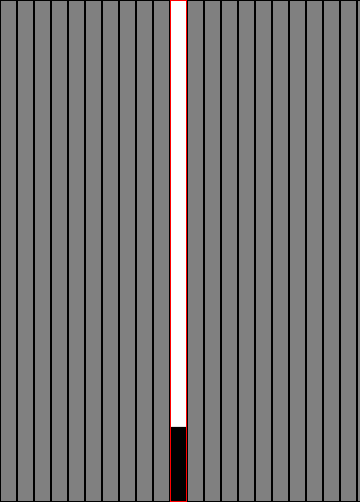
\includegraphics[width=.4\linewidth]{taskb}
				\caption{}
				\label{fig:sub2}
			\end{subfigure}
			\caption{Bars with (a) all rewards hidden and (b) one reward revealed}
			\label{fig:test}
		\end{figure}

	
	\subsection{Experiment 1}
	
	The goal of the first experiment was to test how participants' strategies differed in CMAB, AL, and optimization tasks. Additionally, we tested performance on tasks with a number of different underlying functions.
	
	
	\subsubsection{Participants}
	
	\subsubsection{Procedure}
	
	After giving their informed consent, participants received instructions outlining either the CMAB, AL, or optimization task. Eighty vertical bars were displayed on the screen, with hidden height of each bar determined by one of the following functions:
	
	\begin{equation}
	\begin{split}
	&f_{linear}(x_{i}) = x_{i} \\
	&f_{quadratic}(x_{i}) = -(x_{i}-55)^{2} \\
	&f_{sinc}(x_{i}) = \frac{\sin(x_{i}/2-30.000001)}{x_{i}/2-30.000001}
	\end{split}
	\end{equation}
	normalized between $a \sim U(0,50)$ and $b \sim U(450,500)$. In the CMAB and optimization tasks, participants were given 25 trials to select bars and reveal their heights in a way that increased their scores. In the AL task, participants were first given 25 trials to reveal the heights of bars without their score being affected. After these trials, participants were asked to guess the heights of 25 of bars whose heights they had not chosen to reveal in the previous phase.
	
	\subsubsection{Results}
	
	\subsection{Experiment 1B}
	
	In the first experiment we assume that people are making choices rationally given their model of the underlying function driving the heights of the bars. However, it might be the case that people are either using a model-free policy, marginalizing over some set of functional families, or some other policy. The goal of this experiment was to test whether participant's decisions are rational with respect to information given about the underlying function.
	
	
	\subsubsection{Participants}
	
	\subsubsection{Procedure}  
	
	The CMAB, AL, and optimization tasks and possible underlying functions were identical to those used in Experiment 1. However, participants were given information beforehand indicating the family of the underlying function.
	
	\subsubsection{Results}
	
	\subsection{Experiment 2}
	
	In experiments 1 and 1B, we test whether participants choose their actions rationally, taking into account their goals and the data that they observe. The goal of this experiment is to test whether participants also act rationally across multiple goals, seeking and taking into account information from previous tasks.
	
	\subsubsection{Participants}
	
	\subsubsection{Procedure}  
	
	The CMAB, AL, and optimization tasks and possible underlying functions were identical to those used in Experiment 1 and 1B. However, each participant completed all three tasks one after the other. Additionally, participants were informed that the heights of the bars in all three tasks were determined by a similar function.
	
	\subsubsection{Results}
	
	\section{Discussion}
	
	
	\bibliographystyle{apacite}
	
	\setlength{\bibleftmargin}{.125in}
	\setlength{\bibindent}{-\bibleftmargin}
	
	\bibliography{CogSci_Template}
	
	
\end{document}
